%--------------------------------------------------------------------%
%
% Berkas utama templat LaTeX.
%
% author Petra Barus, Peb Ruswono Aryan
%
%--------------------------------------------------------------------%
%
% Berkas ini berisi struktur utama dokumen LaTeX yang akan dibuat.
%
%--------------------------------------------------------------------%

\documentclass[12pt, a4paper, onecolumn, oneside, final]{report}

%-------------------------------------------------------------------%
%
% Konfigurasi dokumen LaTeX untuk laporan tesis IF ITB
%
% @author Petra Novandi
%
%-------------------------------------------------------------------%
%
% Berkas asli berasal dari Steven Lolong
%
%-------------------------------------------------------------------%

% Ukuran kertas
\special{papersize=210mm,297mm}

% Setting margin
\usepackage[top=3cm,bottom=3cm,left=4cm,right=3cm]{geometry}

\usepackage{mathptmx}

% Judul bahasa Indonesia
\usepackage[indonesian]{babel}
% \usepackage{polyglossia}
% \setdefaultlanguage[variant=indonesian]{malay}

% Format citation
\usepackage[backend=bibtex,citestyle=authoryear]{biblatex}

\usepackage[utf8]{inputenc}
\usepackage{graphicx}
\usepackage{titling}
\usepackage{blindtext}
\usepackage{sectsty}
\usepackage{chngcntr}
\usepackage{etoolbox}
\usepackage{hyperref}       % Package untuk link di daftar isi.
\usepackage{titlesec}       % Package Format judul
\usepackage{parskip}
\usepackage{listings}
\usepackage{parskip}
\usepackage{pdfpages}
% \usepackage{csquotes}
% \usepackage{minted}

% Line satu setengah spasi
\renewcommand{\baselinestretch}{1.5}

% Setting judul
\chapterfont{\centering \Large}
\titleformat{\chapter}[display]
  {\Large\centering\bfseries}
  {\chaptertitlename\ \thechapter}{0pt}
    {\Large\bfseries\uppercase}

% Setting nomor pada subbsubsubbab
\setcounter{secnumdepth}{3}

\makeatletter

\makeatother

% Counter untuk figure dan table.
\counterwithin{figure}{section}
\counterwithin{table}{section}

\usepackage{xcolor}

\definecolor{commentsColor}{rgb}{0.497495, 0.497587, 0.497464}
\definecolor{keywordsColor}{rgb}{0.000000, 0.000000, 0.635294}
\definecolor{stringColor}{rgb}{0.558215, 0.000000, 0.135316}

\definecolor{PigBlue}{RGB}{42, 0, 255}
\definecolor{PigRed}{RGB}{255, 0, 0}

\lstdefinelanguage{Gherkin}{
  morekeywords={When, Then, Given, And, Feature, Scenario, Examples,
                Outline, Fail, Variables, enum, Accepted},
  sensitive=false,
  comment=[l]{\#},
  morestring=[b]',
  morestring=[b]"
}

\lstdefinelanguage{testresult}{
  % morekeywords={SCENARIO, FAIL_SCENARIO, FAILED, SUCCESS},
  keywords=[1]{SCENARIO, SUCCESS},
  keywordstyle=[1]\color{PigBlue},
  keywords=[2]{FAIL_SCENARIO, FAILED},
  keywordstyle=[2]\color{PigRed},
  sensitive=false,
  comment=[l]{\#},
  morestring=[b]',
  morestring=[b]"
}

\lstdefinelanguage{ebnf}{
  morekeywords={:, |, ;},
  alsoletter={:, |, ;},
  morestring=[b]'
}

\lstset{ %
  backgroundcolor=\color{white},   % choose the background color; you must add \usepackage{color} or \usepackage{xcolor}
  basicstyle=\ttfamily\footnotesize,        % the size of the fonts that are used for the code
  breakatwhitespace=false,         % sets if automatic breaks should only happen at whitespace
  breaklines=true,                 % sets automatic line breaking
  aboveskip=15pt,
  belowskip=-30pt,
  captionpos=b,                    % sets the caption-position to bottom
  commentstyle=\color{commentsColor}\textit,    % comment style
  deletekeywords={...},            % if you want to delete keywords from the given language
  escapeinside={\%*}{*)},          % if you want to add LaTeX within your code
  extendedchars=true,              % lets you use non-ASCII characters; for 8-bits encodings only, does not work with UTF-8
  % frame=tb,	                   	   % adds a frame around the code
  keepspaces=true,                 % keeps spaces in text, useful for keeping indentation of code (possibly needs columns=flexible)
  keywordstyle=\color{keywordsColor}\bfseries,       % keyword style
  % language=Python,                 % the language of the code (can be overrided per snippet)
  otherkeywords={*,...},           % if you want to add more keywords to the set
  numbers=left,                    % where to put the line-numbers; possible values are (none, left, right)
  numbersep=5pt,                   % how far the line-numbers are from the code
  numberstyle=\tiny\color{commentsColor}, % the style that is used for the line-numbers
  rulecolor=\color{black},         % if not set, the frame-color may be changed on line-breaks within not-black text (e.g. comments (green here))
  showspaces=false,                % show spaces everywhere adding particular underscores; it overrides 'showstringspaces'
  showstringspaces=false,          % underline spaces within strings only
  showtabs=false,                  % show tabs within strings adding particular underscores
  stepnumber=1,                    % the step between two line-numbers. If it's 1, each line will be numbered
  stringstyle=\color{stringColor}, % string literal style
  tabsize=2,	                   % sets default tabsize to 2 spaces
  title=\lstname,                  % show the filename of files included with \lstinputlisting; also try caption instead of title
  columns=fixed                    % Using fixed column width (for e.g. nice alignment)
}

\begin{filecontents*}{indonesian.lbx}
\ProvidesFile{indonesian.lbx}[2020]

\InheritBibliographyExtras{english}

\DeclareBibliographyStrings{%
  bibliography  = {{Daftar Pustaka}{Daftar Pustaka}},
  and           = {{dan}{dan}},
  in            = {{dalam}{dalam}},
  june          = {{juni}{jun\adddot}},
  january       = {{januari}{jan\adddot}},
  march         = {{march}{mar\adddot}},
  february      = {{februari}{feb\adddot}},
  july          = {{july}{jul\adddot}},
  august        = {{agustus}{aug\adddot}},
  september     = {{september}{sept\adddot}},
  pages         = {{halaman}{hal\adddot}}
}

\endinput

\end{filecontents*}

\makeatletter

\makeatother

\bibliography{references}

\begin{document}

    %Basic configuration
    \title{DSL untuk pengujian keamanan}
    \date{}
    \author{
        Ridho Pratama \\
        NIM 13516032
    }

    \pagenumbering{roman}
    \setcounter{page}{0}

    \clearpage
\pagestyle{empty}

\begin{center}
    \smallskip

    \Large \bfseries \MakeUppercase{\thetitle}
    \vfill

    \Large Tugas Akhir
    \vfill

    \large Disusun sebagai syarat kelulusan tingkat sarjana
    \vfill

    \large Oleh

    \Large \theauthor

    \vfill
    \begin{figure}[h]
        \centering
        % 
\includegraphics[width=0.15\textwidth,natwidth=700,natheight=1021]{resources/cover-ganesha.jpg}
        
\includegraphics[width=0.15\textwidth]{resources/cover-ganesha.jpg}
    \end{figure}
    \vfill

    \large
    \uppercase{
        Program Studi Teknik Informatika \\
        Sekolah Teknik Elektro dan Informatika \\
        Institut Teknologi Bandung
    }

    Agustus 2020

\end{center}

\clearpage

    \clearpage
\pagestyle{empty}

\begin{center}
    \smallskip

    \Large \bfseries \MakeUppercase{\thetitle}
    \vfill

    \Large Laporan Tugas Akhir
    \vfill

    \large Oleh

    \Large \theauthor

    \large Program Studi Teknik Informatika \\
    Sekolah Teknik Elektro dan Informatika \\
    Institut Teknologi Bandung \\

    \vfill
    \normalsize \normalfont
    Telah disetujui dan disahkan sebagai Laporan Tugas Akhir di Bandung, pada tanggal 30 September 2020.

    \vfill
    \setlength{\tabcolsep}{12pt}
    \begin{tabular}{c@{\hskip 0in}c}
        Pembimbing                             \\
         &                                     \\
         &                                     \\
         &                                     \\
         &                                     \\
        Yudistira Dwi Wardhana Asnar ST, Ph.D. \\
        NIP. 19800827 201504 1 002             \\
    \end{tabular}

\end{center}
\clearpage

    \chapter*{Lembar Pernyataan}

Dengan ini saya menyatakan bahwa:

\begin{enumerate}

    \item Pengerjaan dan penulisan Laporan Tugas Akhir ini dilakukan tanpa menggunakan bantuan yang tidak dibenarkan.
    \item Segala bentuk kutipan dan acuan terhadap tulisan orang lain yang digunakan di dalam penyusunan laporan tugas akhir ini telah dituliskan dengan baik dan benar.
    \item Laporan Tugas Akhir ini belum pernah diajukan pada program pendidikan di perguruan tinggi mana pun.

\end{enumerate}

Jika terbukti melanggar hal-hal di atas, saya bersedia dikenakan sanksi sesuai dengan Peraturan Akademik
dan Kemahasiswaan Institut Teknologi Bandung
bagian Penegakan Norma Akademik dan Kemahasiswaan khususnya Pasal 2.1 dan Pasal 2.2.
\vspace{15mm}

Bandung, 06 Desember 2019 \\
Ridho Pratama \\
NIM 13516032


    \pagestyle{plain}

    % \clearpage
\chapter*{ABSTRAK}
\addcontentsline{toc}{chapter}{Abstrak}

%taruh abstrak bahasa indonesia di sini
% \blindtext
\clearpage
    % \clearpage
\chapter*{Abstract}
\addcontentsline{toc}{chapter}{Abstract}

%put your abstract here
% \blindtext

\clearpage
    \chapter*{Kata Pengantar}
\addcontentsline{toc}{chapter}{Kata Pengantar}

Puji syukur penulis sampaikan ke hadirat Allah SWT atas petunjuk serta rahmat-Nya
penulis dapat menyelesaikan Tugas Akhir dengan judul "\thetitle".
Penulis ingin mengucapkan terima kasih kepada pihak-pihak yang telah membantu
penulis dalam proses pengerjaan Tugas Akhir ini:

\begin{enumerate}
  \item Bapak Yudistira Dwi Wardhana Asnar ST, Ph.D. selaku dosen pembimbing yang senantiasa membimbing dan memberikan arahan terhadap penulis.
  \item Bapak Riza Satria Perdana, ST., MT. selaku dosen penguji yang memberikan evaluasi dan masukan dalam pengerjaan Tugas Akhir.
  \item Staf pengajar dari Program Studi Teknik Informatika yang memberikan banyak ilmu serta wawasan untuk mendukung pengerjaan Tugas Akhir.
  \item Ibu Dessi Puji Lestari ST., M.Eng, Ph.D., Ibu Ginar Santika Niwanputri ST. M.Sc.,
        Ibu Dr. Fazat Nur Azizah, ST., M.Sc, dan Bapak Nugraha Priya Utama, ST., M.A., Ph.D.,
        selaku tim koordinator Tugas Akhir yang telah
        menyusun kegiatan terkait Tugas Akhir.
  \item Keluarga penulis, terutama kedua orang tua, yang selalu memberikan dukungan moril untuk penulis.
  \item Teman-teman penulis yang tidak dapat penulis sebutkan satu persatu, sebagai teman seperjuangan penulis yang senantiasa membantu dan menghibur.
  \item Seluruh pihak lain yang ikut membantu penulis yang mungkin tidak tersebutkan sebelumnya.
\end{enumerate}

Akhir kata, semoga Tugas Akhir yang telah penulis susun dapat bermanfaat bagi pembaca.

    \titleformat*{\section}{\centering\bfseries\Large\MakeUpperCase}

    \tableofcontents
    \listoffigures
    \listoftables

    \titleformat*{\section}{\bfseries\Large}
    \pagenumbering{arabic}

    %----------------------------------------------------------------%
    % Konfigurasi Bab
    %----------------------------------------------------------------%
    \setcounter{page}{0}
    \renewcommand{\chaptername}{BAB}
    \renewcommand{\thechapter}{\Roman{chapter}}
    %----------------------------------------------------------------%

    %----------------------------------------------------------------%
    % Dafter Bab
    % Untuk menambahkan daftar bab, buat berkas bab misalnya `chapter-6` di direktori `chapters`, dan masukkan ke sini.
    %----------------------------------------------------------------%
    \chapter{Pendahuluan}

\section{Latar Belakang}

Aplikasi web umum pada saat ini, seperti \textit{e-commerce}, umumnya berfokus pada mekanisme keamanan
seperti \textit{secure transfer protocol}, \textit{paramerter sanitization}, dan menggunakan bermacam skema
kriptografi. Para pengembang aplikasi tersebut lalu beranggapan dengan memberikan fitur keamanan seperti yang
disebutkan sudah cukup, padahal masih banyak kelemahan keamanan aplikasi terjadi pada
tingkat logika bisnis.

\textit{Business Logic Error} (CWE-840) adalah salah satu kelemahan keamanan program yang disebabkan oleh kesalahan pada
tingkat implementasi logika bisnis.
Pengujian kelemahan ini tidak dapat diautomasi oleh kakas otomatis seperti \textit{scanner}
karena bergantung kepada domain dan bisnis aplikasi.
Kelemahan ini juga biasanya terlupakan atau tidak dilakukan karena pada siklus pengembangan aplikasi biasa,
yang diuji hanyalah kebutuhan fungsionalitas aplikasi apakah telah
terimplementasi dengan baik, sementara kelemahan-kelemahan yang mungkin ada tidak teruji.

Pada saat ini, pengujian keamanan biasanya dilakukan setelah pengembangan aplikasi selesai, dan pengujian
dilakukan dengan cara \textit{blackbox} yaitu aplikasi yang telah selesai diberikan bermacam-macam masukan.
Tetapi pengujian dengan cara \textit{blackbox} masih memiliki kelemahan dimana walaupun mungkin bisa menemukan
kelemahan keamanan yang sudah umum diketahui seperti \textit{injection}, cara ini masih jarang menemukan
kelemahan keamanan yang terjadi karena \textit{business logic error} yang biasanya membutuhkan
langkah-langkah yang sangat spesifik dan berbeda tiap aplikasinya.
%Ridho: Please define what is the business logic error... and how it is related to security which one is your main concern

Pengujian keamanan akan menjadi lebih efektif jika diintegrasikan kedalam siklus pengembangan aplikasi.

\section{Rumusan Masalah}

Dari latar belakang tersebut, penulis kemudian merumuskan masalah yaitu:

\begin{enumerate}
    \item Kenapa \textit{business logic error} terjadi?
    \item Kenapa pengujian sulit dilakukan dengan baik walaupun telah menggunakan kerangka pengujian?
    \item Apa yang menyebabkan pengujian keamanan berbeda dengan pengujian fungsionalitas?
    \item Bagaimana cara membuat keamanan mudah diuji pada tahap pengembangan?%dukungan kakas seperti apa yang ....
\end{enumerate}

\section{Tujuan}

Tuliskan tujuan utama dan/atau tujuan detil yang akan dicapai dalam pelaksanaan tugas akhir. Fokuskan pada hasil akhir yang ingin diperoleh setelah tugas akhir diselesaikan, terkait dengan penyelesaian persoalan pada rumusan masalah. Penting untuk diperhatikan bahwa tujuan yang dideskripsikan pada subbab ini akan dipertanggungjawabkan di akhir pelaksanaan tugas akhir apakah tercapai atau tidak.

Subbab sebelum ini telah menjelaskan latar belakang dan rumusan masalah tugas akhir ini.
Karena itu, tujuan dari tugas akhir ini adalah membangun ????? 

\section{Batasan Masalah}

Untuk mencapai tujuan yang telah dijelaskan pada subbab sebelumnya, ????? difokuskan pada hal berikut:

\begin{enumerate}
    \item 
\end{enumerate}

\section{Metodologi}

Metodologi yang digunakan pada pengerjaan tugas akhir ini antara lain:

\begin{enumerate}
    \item 
\end{enumerate}

    \chapter{Tinjauan Pustaka}

Pada bab ini berisi hasil tinjauan pustaka yang menjadi dasar analisa dan perancangan pada BAB III.
Bab ini secara garis besar berisi keamanan perangkat lunak dan pengujiannya,
tantangan pada pengujian perangkat lunak berbasis web, \emph{Domain-Specific Language}, serta BDD dan TDD.

% \begin{enumerate}
%     \item menunjukkan kepada pembaca adanya gap seperti pada rumusan masalah yang memang belum terselesaikan,
%     \item memberikan pemahaman yang secukupnya kepada pembaca tentang teori atau pekerjaan terkait yang terkait langsung dengan penyelesaian persoalan, serta
%     \item menyampaikan informasi apa saja yang sudah ditulis/dilaporkan oleh pihak lain (peneliti/Tugas Akhir/Tesis) tentang hasil penelitian/pekerjaan mereka yang sama atau mirip kaitannya dengan persoalan tugas akhir.
% \end{enumerate}

% \section{Dasar Teori}
%     \subsection{Subbab}
%     \begin{figure}[h]
%         \centering
%         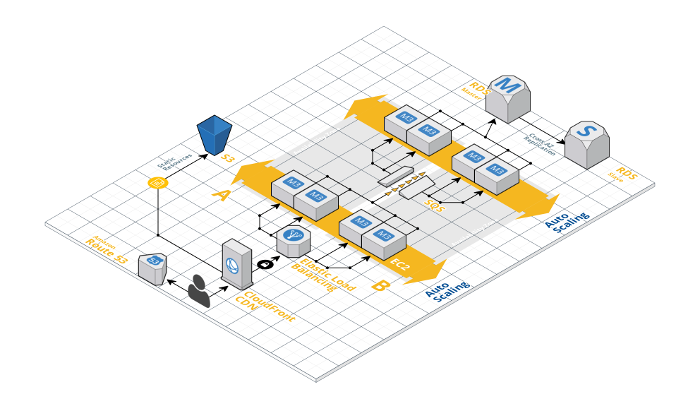
\includegraphics[width=0.8\textwidth]{resources/chapter-2-infrastructure-diagram.png}
%         \caption{Contoh gambar}
%     \end{figure}

\section{Keamanan Perangkat Lunak}

Penggunaan komputer yang semakin hari semakin luas membuat perangkat lunak yang ada semakin besar dan rumit,
yang berarti juga bertambahnya masalah keamanan yang ada pada perangkat lunak tersebut.
Hal ini menyebabkan keamanan perangkat lunak menjadi hal yang semakin penting.

Keamanan perangkat lunak (\emph{software security}) adalah kriteria dimana perangkat lunak tetap bekerja dengan benar
walaupun diserang dengan niat jahat. \emph{Security} berbeda dengan \emph{safety} dimana security fokus terhadap kebenaran
perangkat lunak saat sedang dalam serangan yang dilakukan dengan sengaja, sedangkan \emph{safety} fokus terhadap
kebenaran perangkat lunak saat terjadi kegagalan baik pada tingkat perangkat lunak maupun perangkat keras.

Masalah keamanan perangkat lunak terjadi karena adanya celah atau kecacatan pada perangkat lunak yang dapat
dimanfaatkan oleh penyerang. Celah ini dapat berbentuk kekurangan bawaan pada bahasa pemrograman yang digunakan,
seperti penggunaan \texttt{gets()} pada bahasa C/C++ yang memiliki resiko \emph{buffer overflow},
hingga celah yang terjadi
karena kesalahan pada desain perangkat lunak tersebut. Skala pembuatan perangkat lunak yang semakin besar
dengan proses pengembangan yang melibatkan banyak orang menyebabkan tidak ada satu orang yang paham
cara kerja perangkat lunak secara keseluruhan.

Ada beberapa cara yang dapat dilakukan untuk menanggulangi masalah keamanan perangkat lunak,
namun pada saat ini perlindungan keamanan perangkat lunak dilakukan secara \emph{de facto},
yaitu dengan perlindungan yang diimplementasi setelah aplikasi selesai dikembangkan.
Perlindungan ini biasanya melindungi aplikasi dengan cara memperhatikan data yang masuk
ke dalam aplikasi tidak menimbulkan bahaya atau dapat menyebabkan masalah, pada dasarnya,
perlindungan jenis ini berdasar terhadap pencarian dan mengatasi celah pada aplikasi setelah ditemukan.
Namun, perlindungan perangkat lunak seharusnya mengidentifikasi dan mengatasi masalah dari
dalam perangkat lunak tersebut, sebagai contoh, walaupun ada baiknya mencoba menghadapi serangan
\emph{buffer overflow} dengan membaca \emph{traffic} yang masuk ke dalam aplikasi,
cara yang lebih bagus tentu saja memperbaiki perangkat lunak dari kodenya sehingga
tidak ada kemungkinan \emph{buffer overflow}.

\section{Pengujian Keamanan Perangkat Lunak}

Celah-celah keamanan yang ada pada perangkat lunak selalu menjadi risiko keamanan (\emph{security risk}).
Mengelola risiko keamanan ini menjadi seminimal mungkin adalah salah satu tugas praktisi keamanan perangkat lunak.
Dalam mengelola risiko ini dilakukan beberapa hal, diantaranya:

\begin{itemize}
    \item Membuat kasus penyalahgunaan
    \item Membuat daftar kebutuhan keamanan
    \item Melakukan analisis risiko arsitektur
    \item Membuat perencanaan pengujian keamanan berbasis risiko
    \item Melakukan pengujian keamanan
    \item Melakukan pembersihan setelah terjadinya pelanggaran keamanan
\end{itemize}

Sistem keamanan bukanlah keamanan sistem. Walaupun fitur keamanan seperti \emph{cryptography},
\emph{access control}, dan lain lain memiliki peran penting dalam keamanan perangkat lunak,
keamanan itu sendiri adalah sifat dari sistem secara keseluruhan, bukan hanya dari mekanisme
dan fitur keamanannya. Sebuah \emph{buffer overflow} adalah masalah keamanan, baik itu terletak di dalam
fitur keamanan ataupun di dalam sebuah tampilan non-kritikal.
Karena itu dalam menguji keamanan perangkat lunak memiliki dua macam pendekatan:

\begin{enumerate}
    \item Menguji mekanisme keamanan untuk memastikan bahwa fungsionalitasnya telah diterapkan dengan baik
    \item Melakukan pengujian keamanan berbasis risiko berdasarkan pemahaman dan menyimulasikan pendekatan si penyerang sistem
\end{enumerate}

Banyak \emph{programmer} yang dengan salah mengira bahwa keamanan cukup hanya dengan mengimplementasikan dan
menggunakan fitur-fitur keamanan. Banyak penguji perangkat lunak yang ditugaskan untuk melakukan
pengujian keamanan melakukan kesalahan ini.

Seperti dalam pengujian lainnya, pengujian keamanan perangkat lunak terdiri dari memilih
siapa orang yang akan melakukan pengujian dan apa yang akan dilakukannya.
Dalam memilih orang ada dua kasus tergantung approach yang telah disebutkan,
pada kasus pertama dapat dilakukan oleh staff QA dengan cara pengujian
perangkat lunak seperti biasa untuk melakukan pengujian fungsional
fitur-fitur keamanan sesuai spesifikasi.
Namun pada kasus kedua, staff QA biasa akan kesulitan melaksanakan pengujian berbasis risiko
karena membutuhkan bidang keahlian tertentu.
Pertama, penguji harus dapat berpikir seperti penyerang sistem,
kedua, pengujian keamanan kadang tidak memberikan hasil yang berhubungan langsung dengan
celah keamanan yang ada, sehingga butuh keahlian untuk menginterpretasi dan memahami hasil pengujian.

Kedua, dalam memilih metode pengujian, ada dua metode yang dapat dilakukan.
Pertama dengan cara \emph{White-box} yang dilakukan dengan menganalisis dan memahami
kode serta desain dari program.
Cara ini cukup efektif dalam menemukan kesalahan pemrograman,
dalam beberapa kasus, pengujian ini dapat dilakukan oleh \emph{static analyzer}.
Cara kedua adalah pengujian \emph{Black-box} yang dilakukan dengan cara menguji program
yang sedang berjalan dengan berbagai macam masukan tanpa harus mengetahui masukan program.
Dalam pengujian keamanan, masukan buruk dapat dimasukkan dalam usaha untuk merusak program.
Kedua cara pengujian dapat mengungkapkan adanya risiko keamanan dan kemungkinan eksploitasi.
Masalah yang biasa terjadi dengan pengujian keamanan adalah terkadang organisasi atau perusahaan
tidak memiliki waktu dan sumberdaya untuk melakukan pengujian yang cukup.

Dalam melakukan pengujian keamanan, ada beberapa tantangan yang mungkin dihadapi:
\begin{enumerate}
    \item Adanya efek samping
    
    Dalam melakukan pengujian keamanan dengan pendekatan menguji fungsionalitas perangkat lunak,
    biasanya diberikan sebuah masukan A dan diperiksa apakah perangkat lunak mengembalikan
    hasil B sesuai dengan spesifikasi.
    Namun yang kadang terlupakan bahwa aplikasi dapat memiliki efek samping yang dapat dimanfaatkan
    penyerang sebagai celah keamanan. Salah satu contohnya adalah perangkat utilitas 
    RDISK pada Windows NT 4.0,  yang berfungsi untuk membuat \emph{Emergency Repair Disk}.
    Program ini pada umumnya berjalan baik sesuai spesifikasi, namun saat program berjalan,
    ia membuat sebuah file sementara yang dapat dibaca oleh siapa saja.
    Hal ini berarti pengguna tamu (\emph{guest}) dapat membaca isi file tersebut yang
    termasuk \emph{registry Windows} yang berisi pengaturan tentang sistem yang dapat dimanfaatkan penyerang.

    \item Keadaan Pengujian Keamanan Saat Ini

    Perusahaan yang menyediakan jasa pengujian keamanan biasanya memiliki daftar-daftar celah yang umum ada.
    Mereka biasanya hanya menggunakan daftar tersebut untuk membuat rencana pengujian.
    Cara seperti ini biasanya tidak akan dapat menemukan celah-celah keamanan yang baru.

    \item Ketidakamanan dan kegagalan aplikasi penunjang

    Perangkat lunak modern berjalan pada sistem yang saling bergantung satu sama lain,
    dimana satu aplikasi menggunakan puluhan \emph{library} dan berkomunikasi dengan
    beberapa komponen lainnya.
    Hal ini dapat menimbulkan dua masalah.
    Pertama, aplikasi dapat memiliki celah dari salah satu komponen yang ia gunakan.
    Kedua, sebuah komponen yang digunakan untuk menyediakan fungsionalitas keamanan
    dapat saja pada suatu saat rusak dan berhenti bekerja.

    \item Masukan tidak terkira dari pengguna

    Masukan dari pengguna adalah salah satu sumber celah yang paling umum dan paling mudah dieksploitasi.
    Beberapa contoh yang umum digunakan adalah masukan yang panjang, karakter spesial, dan nilai-nilai khusus.
    Salah satu contoh celah yang terjadi dari masukan pengguna ini adalah \emph{buffer overflow},
    yang memungkinkan penyerang menyisipkan kode pada masukan yang sangat panjang,
    hingga tidak bisa ditampung \emph{buffer} dan dijalankan oleh komputer. 

    \item Ketidakamanan desain

    Banyak celah keamanan terjadi sejak perangkat lunak masih dalam tahap desain.
    Kadang celah tersebut tidak bisa langsung diketahui karena terjadi setelah semua
    bagian sistem selesai dirancang namun gabungan dari keseluruhan sistem tersebut
    menyebabkan adanya celah.
    Kadang celah juga terjadi pada test interface, yaitu bagian program yang sengaja
    disisipkan dan memberi celah untuk pengujian, namun tidak dihilangkan saat program akan dirilis.

    \item Ketidakamanan implementasi

    Walaupun spesifikasi perangkat lunak telah didesain sebaik mungkin dengan
    mempertimbangkan berbagai macam aspek keamanan,
    celah tetap dapat terjadi karena implementasi perangkat lunak yang tidak sempurna.

\end{enumerate}

\section{Tantangan Dalam Pengujian Aplikasi \emph{Web}}

Perangkat lunak berbasis web adalah salah satu jenis perangkat lunak paling umum pada saat ini.
Perangkat lunak ini menjadi tulang belakang dari komunikasi di dunia dan banyak hal-hal
yang membutuhkan keamanan tinggi menggunakan perangkat lunak berbasis web seperti perbankan.
Hal seperti menyebabkan perangkat lunak berbasis web menjadi salah satu target yang empuk untuk
dimanfaatkan celah dan kekurangannya. Sifat dari aplikasi web yang dinamis, kompleks, dan
selalu berubah-ubah membuat semakin mudahnya muncul celah baru pada aplikasi web jika tidak diperhatikan.

Beberapa masalah umum yang ada pada perangkat lunak berbasis web adalah:
\begin{enumerate}
    \item Autentikasi: memastikan pengguna yang meminta data adalah benar pengguna tersebut
    \item Autorisasi: memastikan pengguna boleh melakukan hal yang dilakukannya.

    \item \emph{Cross-site scripting}:
    celah dimana penyerang dapat memasukkan kode jahat ke halaman web yang dijalankan di browser pengguna lain.

    \item \emph{SQL injection}:
    celah dimana disisipkannya kode jahat di dalam perintah SQL yang kemudian dijalankan oleh \emph{database}.

    \item \emph{Cross-site request forgery}:
    celah dimana sebuah \emph{website} dapat dieksploitasi untuk mengirimkan perintah palsu dari sebuah user.

    \item \emph{Malicious file execution}:
    aplikasi web menjalankan kode jahat yang berada di sebuah file bebas
\end{enumerate}

Beberapa tantangan dalam melakukan pengujian keamanan terhadap aplikasi web adalah:
\begin{enumerate}
    \item Butuhnya pengembangan kakas yang dapat mengotomatisasi pengujian aplikasi web.
    
    \item Pengembangan aplikasi web yang dinamis dan \emph{Rich Content} seperti \emph{Single-Page Application}
    mempersulit \emph{crawling} halaman web sehingga bisa saja ada state halaman yang
    tidak bisa dicapai oleh kakas pengujian.

    \item Bahasa pemrograman yang digunakan pada implementasi tidak memiliki fitur yang
    dapat memaksa penggunaan aturan keamanan yang dapat menyebabkan bahaya terhadap keamanan
    dan integritas data pengguna.
\end{enumerate}

\section{\emph{Domain-Specific Language}}

\emph{Domain-Specific Language} (DSL) adalah bahasa pemrograman berkemampuan terbatas yang
berfokus pada suatu domain tertentu.

Dari definisi diatas, ada empat poin penting:

\begin{enumerate}
    \item DSL dapat digunakan untuk memerintahkan komputer. Seperti bahasa pemrograman lainnya,
    DSL haruslah bisa untuk dipahami manusia, tetapi masih mungkin diolah oleh komputer.

    \item DSL adalah bahasa pemrograman komputer. Hal ini berarti DSL harus terasa seperti
    bahasa yang dimana kemampuannya tidak hanya muncul dari masing-masing ekspresinya,
    tetapi juga saat ekspresi-ekspresi tersebut digabungkan.

    \item Bahasa pemrograman umum (\emph{General Purpose Programming Language}) memiliki banyak fitur.
    Hal ini membuatnya sangat berguna, namun menjadi susah untuk dipelajari dan digunakan.
    DSL dengan kemampuannya yang terbatas hanya memiliki fitur-fitur minimum yang dibutuhkan untuk domainnya.

    \item Sebuah bahasa dengan kemampuan terbatas hanya akan berguna jika ia memiliki
    fokus yang jelas terhadap sebuah domain kecil.
\end{enumerate}

DSL terbagi menjadi dua kategori, yaitu:

\begin{enumerate}
    \item \emph{External DSL}

    DSL eksternal adalah bahasa yang terpisah dari bahasa utama aplikasi.
    Biasanya, DSL eksternal memiliki syntaxnya sendiri, namun kadang dapat menggunakan
    bahasa lain seperti XML. Sebuah kode pada DSL eksternal biasanya akan diproses oleh
    aplikasi utama. Beberapa contoh DSL eksternal adalah Regex, SQL, awk, sed.

    \item \emph{Internal DSL}
    
    DSL internal adalah sebuah cara tertentu untuk menggunakan sebuah bahasa.
    Sebuah DSL internal ditulis dalam bahasa yang sama dengan bahasa utama aplikasi,
    namun hanya menggunakan sebagian fitur bahasa untuk mengurusi bagian kecil 
    dari keseluruhan sistem. Salah satu bahasa yang memiliki banyak DSL internal adalah Ruby,
    karena struktur Ruby yang ekspresif memudahkan dibuatnya DSL.
    Web framework Rails yang ditulis dengan Ruby adalah salah satu contoh DSL.
\end{enumerate}

DSL adalah sebuah alat yang memiliki fokus yang jelas dan hanya mengurusi suatu
aspek kecil tertentu. Sebuah aplikasi bisa saja menggunakan banyak DSL untuk mengurusi
berbagai aspek sistemnya. Beberapa kelebihan menggunakan DSL adalah:

\begin{enumerate}
    \item Meningkatkan produktivitas

    Salah satu daya tarik utama dari DSL adalah ia menyediakan cara untuk menyampaikan
    sebuah maksud sebuah sistem dengan lebih jelas.
    Hal ini menyebabkan programmer lebih mudah memahami maksud dan
    tujuan sebuah kode dan sistem.

    \item Merepresentasikan pengetahuan domain dengan lebih baik

    DSL dapat didesain sedemikian mungkin untuk merepresentasikan dan mengabstraksikan
    suatu domain tertentu, sehingga
    bisa digunakan bukan hanya oleh \emph{programmer} saja, tetapi juga oleh ahli domain tersebut.
\end{enumerate}

Sementara kekurangan menggunakan DSL adalah:

\begin{enumerate}
    \item \emph{Language cacophony}
    
    Beberapa komplain yang sering didengar saat menggunakan DSL adalah \emph{language cacophony},
    dimana bahasa biasanya sulit untuk dipelajari, sehingga menggunakan banyak bahasa akan lebih
    sulit dari pada menggunakan satu bahasa. Kebutuhuan untuk mempelajari banyak bahasa menyebabkan
    sulit untuk mengerjakan proyek dan menambah orang baru kedalam proyek.

    Namun dari komplain ini, banyak orang yang berpikiran bahwa mempelajari sebuah DSL akan sesulit
    mempelajari bahasa pemrograman general biasa. Tetapi, DSL sebenarnya lebih mudah dipelajari
    karena keterbatasannya.

    \item Biaya pembuatan
    
    Seperti semua bagian dari program, DSL juga merupakan program yang harus dibuat dan dipelihara.
    Tentu saja hal ini dapat menambah biaya yang harus dikeluarkan. Biaya pembuatan DSL juga dapat
    lebih tinggi karena tim yang ada tidak terbiasa membuat DSL sehingga harus belajar lagi, yang
    juga dapat menambah biaya.

\end{enumerate}

% TODO: BDD Testing and Gherkin
    \chapter{Analisis dan Perancangan}

\section{Analisis \emph{Business Logic Error}}

\subsection{Analisis}

Celah keamanan bisa terjadi karena pada pada siklus pengembangan perangkat lunak
biasa, \emph{programmer} hanya fokus terhadap kebutuhan fungsional,
memerhatikan aspek keamanan. Hal ini juga menjadi penyebab dari BLE.
BLE, secara spesifik, terjadi karena beberapa hal.
Pertama, adanya perbedaan kecil dari step sebuah skenario fitur, misal pada state awal,
jika fitur
menambahkan barang ke dalam keranjang membutuhkan state awal user untuk telah login,
apa yang terjadi jika penambahan barang dilakukan saat user belum login.
Kedua, saat \emph{business} menuliskan deskripsi skenario business logic,
yang bisa dituliskan dengan mudah biasanya hanya skenario positif dimana
fitur berjalan sebagaimana seharusnya. Namun, kasus-kasus dimana fitur
tidak berjalan sesuai dengan seharusnya tidak dituliskan, karena bagi orang bisnis,
hal itu adalah sesuatu hal yang mereka rasakan \emph{obvious}.
BLE terjadi saat \emph{programmer} dan \emph{tester} yang tidak memiliki
pengetahuan domain sebanyak orang bisnis, tidak mengetahun asumsi-asumsi tersebut dan lupa
untuk mengujinya.

Dalam masa pengembangan suatu fitur, \emph{programmer} bisa saja memikirkan
apa saja kemungkinan variasi dari nilai-nilai suatu fitur. Programmer
dapat mencoba mengakomodasi semua variasi itu, tetapi pengetahuan tentang
adanya variasi tersebut mungkin hanya teringat pada saat mengerjakan
fitur tersebut. Sehingga di akhir pada saat melakukan \emph{acceptance test},
\emph{tester} tidak tau tentang variasi ini dan tidak mengujinya.
Bahkan, bisa saja \emph{programmer} yang sedang mengerjakan fitur tersebut
lupa terhadap variasi tersebut beberapa hari kemudian.

\emph{Tester} bisa saja mencoba memikirkan banyak \emph{abuse case} pada saat
akan melakukan pengujian suatu fitur, dan tentu menggunakan \emph{tester} yang
berbeda dengan orang yang melakukan implementasi akan menghilangkan beberapa
subjektifitas dalam \emph{abuse case}. Namun, sang \emph{programmer} tadi yang
sempat memikirkan kasus-kasus variasi tentu juga memiliki pengetahuan yang banyak
tentang fitur tersebut, namun tidak menuliskan kasus-kasus tersebut karena merasa
melakukan pengujian adalah pekerjaan \emph{tester}, merasa menuliskan kasus pengujian
adalah hal yang sulit dan hal lainnya seperti di kejar
deadline, dan lain lain. \emph{Insight} dari \emph{programmer ini} tentu berharga,
namun tidak terdokumentasi dan hilang.

\subsection{Language Requirement}

Dari analisis di atas kita dapat mengetahui kebutuhan-kebutuhan bahasa
agar dapat melakukan pengujian efektif terhadap BLE, yaitu:

\begin{enumerate}
  \item Mudah

        Bahasa yang akan dibuat haruslah mudah dipahami, sehingga semua pihak tetap
        bisa memahaminya, dan mudah ditulis, sehingga \emph{programmer} yang ``sibuk''
        terdorong untuk menulis kasus pengujian.

  \item Bisa menyatakan kegagalan

        Pada pengujian fungsionalitas, kita hanya menuliskan kasus-kasus positif
        dimana skenario berjalan dengan benar. Namun untuk pengujian BLE,
        menuliskan dan melakukan pengujian dimana skenario tidak berjalan dengan benar
        haruslah sama mudahnya dengan skenario yang benar.

  \item Bisa menyatakan variansi

        Seperti yang telah disebutkan di atas, salah satu penyebab dari BLE adalah
        adanya variansi-variansi dari skenario.
        Bahasa yang akan dibuat haruslah dapat menyatakan variansi ini dengan mudah.
        Hal ini dapat mengurangi duplikasi dan meningkatkan pemahaman bersama.
\end{enumerate}



\section{Kondisi Gherkin}

Kita dapat membandingkan kebutuhan bahasa yang telah dianalisa dengan keadaan Gherkin pada saat ini.

\subsection*{Mudah}

Gherkin yang menggunakan bahasa manusia sudah mudah dimengerti, dan kita ingin agar bahasa
baru yang akan dibuat dapat dipahami dan ditulis semudah Gherkin.

\subsection*{Bisa menyatakan kegagalan}

Pada saat ini, penulisan \emph{step} pada Gherkin lebih berorientasi terhadap
kasus sukses. Misalkan untuk step \texttt{Then the basket should have items in it},
dapat memiliki step gagal berupa \texttt{Then the basket should not have items in it}.
Secara semantik hal dua tadi adalah kebalikan, dimana logika pengujian
sama, berbeda namun di akhir kode \emph{step definition}. Hal ini
menyebabkan banyaknya duplikasi kode \emph{step definition} dan membuat \emph{programmer} malas untuk
melakukannya.
Duplikasi ini dikarenakan setiap kode \emph{step definition} dari Gherkin dianggap
sukses/\emph{passing} jika tidak ada exception yang terjadi.
Kita ingin mengurangi duplikasi dan mengingkatkan \emph{code reuse}.
Kita ingin agar kode \emph{step definition} dari step \texttt{Then the basket should have items in it}
dapat digunakan untuk skenario sukses ataupun gagal.

Bahasa yang akan dibuat haruslah dapat menyatakan kegagalan dalam bagian bahasanya.
Seperti Gherkin, namun memiliki keyword yang menyatakan bahwa suatu skenario
harus lah gagal.

\subsection*{Bisa menyatakan variansi}

Gherkin pada saat ini memiliki fitur \emph{scenario outline} yang dapat menyatakan banyak skenario yang mirip
hanya dalam satu skenario saja dengan menggunakan template dan tabel.
\emph{Scenario outline} dapat memenuhi kebutuhan bahasa untuk menyatakan variansi.

Namun fitur ini dapat dikembangkan dengan menambah kemampuan untuk menyatakan domain/tipe data suatu variabel, misalkan
domain \texttt{integer}, \texttt{positive}, \texttt{string}, \emph{enum}, dan lain lainnya.
Hal ini membuat deklarasi variansi lebih singkat dan padat.
Kemampuan ini juga dapat digabungkan dengan poin sebelumnya.
Untuk \emph{Scenario outline}, kita dapat menyatakan tabel \emph{example} dengan kombinasi-kombinasi varian yang harus gagal.
Untuk domain variabel, kita dapat menyatakan nilai mana saja yang harus gagal.


\section{Rancangan Solusi}

Dari bagian sebelumnya, pada bagian ini akan dibahas desain bahasa untuk fitur yang dianalisa
dan cara implementasi.

\subsection{Menyatakan Kegagalan}

Pada saat ini Gherkin hanya menyatakan \textit{step} yang positif seperti
"barang sukses ditambahkan ke dalam keranjang", namun butuh mendeskripsikan \textit{step function}
lagi untuk negatif \textit{step} tersebut seperti "barang gagal ditambahkan ke dalam keranjang" atau
"barang tidak sukses ditambahkan ke dalam keranjang".

Untuk pembahasan fitur ini, kita akan mengacu pada kode Gherkin dibawah:
\begin{lstlisting}[language=gherkin]
Feature: keranjang
  Scenario: menambahkan barang ke dalam keranjang
    Given user telah login
    When user memasukkan 1 barang
    Then ada 1 barang di dalam keranjang
\end{lstlisting}

Untuk desain fitur Failure dapat kita lakukan beberapa hal.

\subsubsection{Scenario Outline}
Screnario di atas memiliki initial state dimana user telah login.
Programmer dapat menambahkan satu skenario lagi untuk keadaan dimana user gagal login, seperti:
\begin{lstlisting}[language=gherkin]
Feature: keranjang
  Scenario: menambahkan barang ke dalam keranjang
    Given user telah login
    When user memasukkan 1 barang
    Then sukses ada 1 barang di dalam keranjang
  Scenario: user belum login menambahkan barang 
    Given user belum login
    When user memasukkan 1 barang
    Then gagal ada 1 barang di dalam keranjang
\end{lstlisting}

Fitur \textit{Scenario Outline} dari Gherkin dapat dimanfaatkan untuk memperpendek skenario ini menjadi

\begin{lstlisting}[language=gherkin]
Feature: keranjang
  Scenario Outline: menambahkan barang ke dalam keranjang
    Given user <login state> login
    When user memasukkan 1 barang
    Then <result state> ada 1 barang di dalam keranjang

    Examples:
      | login state | result state |
      | sudah       | sukses       |
      | belum       | gagal        |
\end{lstlisting}

Dengan begini, masalah duplikasi skenario terselesaikan namun programmer tetap
harus mendefinisikan tabel pada scenario outline, dan \textit{step} yang didefinisikan
pada bagian \textit{Then} tetap harus dibuat \textit{step definition}nya.

\subsubsection{Variansi}

Pada bagian sebelumnya telah

% \section{Perbedaan Pengujian Fungsionalitas dan \emph{Business Logic Error}}

% Pengujian untuk fungsionalitas dan untuk keamanan memiliki perbedaan. 
% Pada pengujian fungsionalitas, yang dibutuhkan hanyalah untuk menguji apakah
% fungsionalitas telah terimplementasikan dengan benar.
% Namun pada pengembangan aplikasi terkadang secara tidak sengaja ada fungsionalitas
% tambahan yang bisa menjadi celah keamanan yang sering terlupakan untuk diuji.
% Salah satu macam dari celah ini adalah \emph{business logic error}.

% Pengujian untuk \emph{business logic error} dilakukan dengan memperhatikan tiap-tiap fungsionalitas
% yang diimplementasikan dalam program dan menguji kemungkinan variasi keadaan pada
% fungsionalitas tersebut. Salah satu contohnya adalah pada aplikasi \emph{e-commerce} yang memiliki
% fitur keranjang. Pada fungsionalitas "bisa menambahkan barang ke dalam keranjang", dapat memiliki
% prasyarat bahwa user hanya bisa memasukkan barang ke dalam keranjang jika sudah login, dan skenario
% ini lah yang biasa diuji pada pengujian fungsionalitasnya. Namun untuk \emph{business logic error} 
% terjadi saat asumsi-asumsi normal itu tidak berlaku seperti, bagaimana jika user belum login,
% bagaimana jika user memasukkan -1 barang, dan lain-lain.

% Salah satu cara pengujian fungsional dapat diintegrasikan ke dalam siklus pengembangan aplikasi
% adalah dengan menggunakan kerangka pengujian BDD atau TDD. Kerangka ini mengharuskan \emph{programmer}
% untuk menulis spesifikasi dan kasus uji sebelum mulai menulis kode.
% Salah satu dari kerangka ini adalah Cucumber BDD, beserta bahasa yang ia gunakan untuk mendeskripsikan
% kasus uji, yaitu Gherkin.

% Gherkin adalah bahasa yang digunakan untuk mendeskripsikan spesifikasi fungsionalitas
% aplikasi. Spesifikasi ini ditulis per-skenario, dimana tiap-tiap skenario dibagi menjadi
% langkah-langkah simpel yang menjelaskan skenario tersebut. Dari Gherkin ini kemudian
% digunakan oleh Cucumber untuk menjalankan pengujian.

% Gherkin jika digunakan dengan baik dapat membantu implementasi dan
% pengujian fungsionalitas aplikasi. Tetapi, Gherkin masih belum bisa digunakan untuk melakukan
% pengujian \emph{business logic error} dengan mudah.
% Dalam siklus pengembangan perangkat lunak, \emph{programmer} biasanya memiliki
% banyak deadline yang harus dikejar, sehingga pengembangan hanya seperti ``kejar tayang'',
% yang menyebabkan \emph{programmer} hanya memperhatikan sisi fungsionalitas dari perangkat lunak.
% Adanya kesulitan dalam melakukan pengujian keamanan dapat membuat
% \emph{programmer} semakin enggan melakukannya, walaupun mungkin pada saat
% melakukan rancangan solusi dan implementasi \emph{programmer} juga memikirkan kemungkinan
% kesalahan atau celah keamanan yang mungin terjadi.
% Jika kesulitan-kesulitan tersebut dapat dihilangkan maka \emph{programmer} akan
% dapat langsung menuliskan kasus-kasus pengujian keamanan.
% Namun ada dua hal yang dapat ditambahkan
% ke dalam Gherkin untuk mempermudah pengujian \emph{business logic error}, yaitu kemampuan untuk
% mengecek kegagalan, dan kemampuan untuk mendefinisikan banyak state/value dengan mudah.

% \section{Failure}

% Kekurangan pertama Gherkin yang akan dibahas adalah ketidakmampuan untuk
% menyatakan suatu skenario harus gagal.
% Hal ini terjadi karena desain Gherkin yang bertujuan untuk menguji fungsionalitas saja,
% sehingga setiap step Gherkin dianggap benar jika tidak ada \emph{error}/\emph{exception}
% dari fungsi implementasi stepnya.
% Namun untuk pengujian \emph{business logic error}, dibutuhkan kemampuan untuk menyatakan
% bahwa suatu skenario atau stepnya harus gagal, dan pengujian dianggap tidak lolos
% jika skenario tersebut tidak gagal (dalam bentuk \emph{error/exception}).

% Dengan kemampuan untuk mendefinisikan bahwa suatu skenario harus gagal,
% \emph{programmer} dimudahkan untuk membuat lebih banyak test case
% yang menguji keamanan \emph{business logic error}.
% Pada saat ini pengujian kasus yang harus gagal bisa dilakukan
% pada Gherkin, namun dengan mendefinisikan suatu \emph{step} sebagai negatif.
% Hal ini dapat menyebabkan banyak duplikasi kode-kode yang pada dasarnya
% melakukan hal yang sama.

% \section{Variable Domain}

% Pada saat ini, Gherkin memiliki fitur \emph{scenario outline}
% untuk mendefinisikan sebuah \emph{template} skenario,
% didalamnya dapat digunakan \emph{placeholder} variabel yang dapat didefinisikan
% dalam sebuah tabel.
% Penggunakan \emph{scenario outline} memungkinkan \emph{programmer} untuk
% mendefinisikan banyak skenario yang mirip dengan variasi nilai dengan mudah.

% Fitur ini dapat dikembangkan dengan menambahkan fungsionalitas dimana 
% variabel-variabel yang digunakan dapat diberikan tipe data,
% sehingga memiliki domain yang jelas. Tipe data dapat berupa \emph{enum string},
% \emph{integer}, \emph{positive integer}, dan lain lain.
% Fitur ini digabungkan dengan kemampuan untuk menyatakan
% skenario yang harus gagal dapat mempermudah \emph{programmer}
% dalam mendeskripsikan kasus-kasus pengujian keamanan bersamaan dengan
% menulis kasus pengujian fungsionalitas.
    % \chapter{Implementasi}

\section{Detail Implementasi}

Seluruh komponen dibuat dengan menggunakan bahasa python. Kakas dibuat dengan bentuk library python
sehingga dapat diinstall dengan mudah menggunakan \emph{pip}. Kakas didesain untuk menguji
program yang juga ditulis dengan bahasa python. Kode implementasi dan pengujian terdapat
di repositori \\\url{https://gitlab.informatika.org/rid9/thesis}.

\subsection{Parser}

Komponen \emph{parser} berfungsi untuk membaca \emph{file} fitur dan menguraikan isinya menjadi
struktur data yang dapat diolah. Komponen ini hanya menghasilkan skenario dalam bentuk dasar
yang hanya berisi step-step, sehingga semua bentuk skenario yang lebih kompleks
seperti \emph{scenario outline} akan diuraikan terlebih dahulu menjadi semua kemungkinan
kombinasi skenario dasarnya. Sebagai contohnya adalah

\begin{lstlisting}[language=gherkin]
Scenario Outline: menambahkan barang ke dalam keranjang
  Given user <login state> login
  When user memasukkan 1 barang
  Then <result state> ada 1 barang di dalam keranjang
  Examples:
    | login state | result state |
    | sudah       | sukses       |
    | belum       | gagal        |
\end{lstlisting}

Kode diatas akan diuraikan menjadi skenario dasar dengan bentuk

\begin{lstlisting}[language=gherkin]
Scenario: menambahkan barang ke dalam keranjang (1)
  Given user sudah login
  When user memasukkan 1 barang
  Then sukses ada 1 barang di dalam keranjang
Scenario: menambahkan barang ke dalam keranjang (2)
  Given user belum login
  When user memasukkan 1 barang
  Then gagal ada 1 barang di dalam keranjang
\end{lstlisting}

Perubahan ini berfungsi agar komponen \emph{runtime} hanya perlu tahu cara menjalankan
skenario dasar saja sehingga lebih simpel, dan juga memperbanyak jumlah step yang diketahui
oleh kakas sehingga dapat membangkitkan skenario acak yang lebih beragam.

Kode penguraian menggunakan arsitektur \emph{Parsing Expression Grammar} (PEG), dimana
pada arsitektur ini setiap \emph{non-terminal} seperti \texttt{scenario, scenarioOutline, feature}
yang ada dalam \emph{grammar} pada \ref{sec:struktur-bahasa} dibentuk menjadi fungsi-fungsi
yang dapat disusun, sehingga kode penguraian mirip dengan \emph{grammar}. Fungsi-fungsi
ini memiliki tipe parameter dan kembalian yang sama sehingga
dapat dikomposisikan menghasilkan fungsi yang lebih kompleks. Pada psudeocode dibawah
akan diilustrasikan kode penguraian untuk grammar \texttt{scenario} simpel.

\begin{lstlisting}[language=python]
# fungsi kombinator
def optional(func)      # func?
def zero_or_more(func)  # func*
def one_or_more(func)   # func+
def or(func1, func2,..) # func1 | func2 | ..
def literal(string)     # "string"
def parseString(input)  # string
def newline(input):
  return literal("\n")(input)

def parseStepKeyword:
  return or(literal("given"), literal("when"), literal("then"))

def parseStepLine(input):
  keyword, input = parseStepKeyword(input)
  line, input = parseString(input)
  _, input = newline(input)
  return Step(keyword, line), input

def parseScenarioKeyword:
  return or(
    literal("scenario"),
    literal("fail scenario")
  )

def parseStepLines(input):
  return one_or_more(parseStepLine)(input)

def parseScenario(input):
  keyword, input = parseScenarioKeyword(input)
  _, input = literal(":")(input)
  desc, input = parseString(input)
  _, input = newline(input)
  steps, input = parseStepLines(input)

  return Scenario(keyword, desc, steps), input
\end{lstlisting}


\subsection{Importer}

Importer berfungsi untuk membaca \emph{file} step descriptor yang ditulis dalam python.
Importer menghasilkan kumpulan fungsi \emph{step descriptor} yang akan digunakan untuk
menjalankan step-step yang telah didefinisikan dari skenario.

Importer akan membaca semua file python yang ada dalam folder fitur, lalu mencoba untuk
mencari semua fungsi yang merupakan step descriptor yang memiliki \emph{decorator} python.
Semua fungsi ini lalu dikumpulkan dan diteruskan ke komponen \emph{runtime}.
Cara kerja importer secara simpel digambarkan oleh \emph{psudeocode} berikut:

\begin{lstlisting}[language=python]
def feature_folder
def step_descriptors = []

for file in feature_folder:
  file_objects = import(file)
  for function in file_objects.functions:
    if function is step descriptor:
      step_descriptors.add(function)

return step_descriptors
\end{lstlisting}

\subsubsection{API}

Komponen ini adalah bagian dari kakas \emph{library} yang digunakan oleh user untuk menulis
\emph{step descriptor}. Bagian ini meng-\emph{export} decorator-decorator yang disediakan.
Decorator ini berfungsi untuk menandai fungsi sebagai \emph{step descriptor} sehingga dapat
dibedakan dari fungsi biasa oleh \emph{importer}. Cara kerja descriptor dan contoh penggunaannya
digambarkan oleh \emph{psudeocode} berikut:

\begin{lstlisting}[language=python]
def step_decorator(keyword, function):
  mark function as step decorator
  return function
def given(func):
  return step_decorator("given", func)
def when(func):
  return step_decorator("when", func)
def then(func):
  return step_decorator("then", func)

# contoh penggunaan
@given("user awalnya punya {num} kue")
def step1(num):
  user.kue = num

@when("user memakan {num} kue")
def step2(num):
  user.kue -= num

@then("user sisa kue {num}")
def step3(num):
  assert user.kue == num
\end{lstlisting}


\subsection{Runtime}

Runtime berfungsi untuk menjalankan pengujian. Runtime menerima hasil dari parser dan importer,
mencocokkan step-step dalam skenario dengan fungsi \emph{step descriptor} yang cocok,
dan kemudian menjalankan skenario pengujian.

Runtime menghasilkan laporan penjalanan pengujian. Laporan ini berisi skenario apa saja
yang berhasil dan gagal. Laporan ini juga berisi penyebab kegagalan skenario dalam
bentuk catatan exception.

Bagian runtime juga berfungsi untuk membangkitkan skenario acak dari \emph{step} yang telah ada
dan menjalankannya.




\section{Validasi}

Pada tugas akhir ini akan digunakan kosa kata validasi untuk membedakan pengujian yang dilakukan oleh kakas ini terhadap program user (pengujian)
dengan pengujian yang dilakukan terhadap kakas ini (validasi).

\subsection{Tujuan Validasi}

Validasi dilakukan dengan tujuan untuk mengevaluasi apakah kakas yang dibuat dapat digunakan dengan
baik dan membantu programmer untuk menemukan kelemahan keamanan pada perangkat lunak.
Dalam validasi juga ditentukan apakah kakas yang dibuat mudah digunakan atau masih ada kekurangan.

\subsection{Skenario Validasi}

Validasi dilakukan dengan cara membuat file fitur untuk suatu proyek tertentu secara perlahan hingga semua fitur
telah diuji secara BDD. Proyek yang akan diuji adalah proyek sistem perwalian mahasiswa dimana terdapat data mahasiswa, ipk,
serta sks yang akan diambil. Sistem memiliki business logic dimana sks hanya bisa diambil menurut ipk, jika ipk kurang sama dari
2 maka mahasiswa tidak dapat mengambil lebih dari 20 sks. Sistem juga akan mengecek bahwa mahasiswa tidak bisa disetujui
jika belum melakukan pembayaran.

Validasi dimulai dengan membuat proyek kosong python. Kemudian dilanjutkan dengan menulis \emph{file feature}
dengan satu skenario. Kemudian \emph{step definition} dibuat untuk semua step yang dibuat. Setelah \emph{file}
pengujian dibuat dilanjutkan dengan membuat program yang mengimplementasikan skenario tersebut. Jika semua
test untuk skenario telah berjalan dengan baik, dibuat \emph{file feature} untuk skenario selanjutnya.
Dalam pengerjaan juga dilakukan \emph{refactor} dengan fitur yang telah didesain.

\subsection{Hasil Validasi}

Berikut adalah kode gherkin yang digunakan untuk validasi program.

\begin{lstlisting}[language=gherkin]
Variable:
    paid status: enum true, false
    approve status: enum true, false

Feature: mahasiswa feature
    Scenario: create mahasiswa default
        Given prepare mahasiswa 001
        When create mahasiswa 001
        Then mahasiswa 001 exists
    
    Fail Scenario: create mahasiswa fail
        Given prepare mahasiswa 002
        When create mahasiswa 001
        Then mahasiswa 003 exists

    Scenario Outline: sks must correct for approve
        Given prepare mahasiswa 001
        Given mahasiswa 001 have paid true
        Given mahasiswa 001 ipk is <ipk>
        Given mahasiswa 001 ambil sks <sks>
        Given mahasiswa 001 approve <approve>
        When create mahasiswa 001
        Then mahasiswa 001 exists

        Example:
            | ipk   | sks   | approve   |
            | 4     | 24    | true      |
            | 2     | 20    | true      |
            # bisa tidak approve walaupun sks benar
            | 4     | 24    | false     |

        Fail Example:
            | ipk   | sks   | approve   |
            | 2     | 24    | true      |


    Scenario: must have paid before approve
        Given prepare mahasiswa 001
        Given mahasiswa 001 have paid <paid status>
        Given mahasiswa 001 approve <approve status>
        When create mahasiswa 001
        Then mahasiswa 001 exists

        Variable Rejected:
            | paid status  | approve status  |
            | false        | true            |


    Scenario Outline: ipk range
        Given prepare mahasiswa 001
        Given mahasiswa 001 ipk is <ipk>
        When create mahasiswa 001
        Then mahasiswa 001 exists
        Example:
            | ipk   |
            | 0     |
            | 2     |
            | 4     |
        Fail Example:
            | ipk  |
            | -1.0 |
            | 5.0  |

    
    Scenario Outline: sks range
        Given prepare mahasiswa 001
        Given mahasiswa 001 ipk is 4
        Given mahasiswa 001 ambil sks <sks>
        When create mahasiswa 001
        Then mahasiswa 001 exists

        Example:
            | sks   |
            | 0     |
            | 12    |
            | 24    |
        Fail Example:
            | sks   |
            | -1    |
            | 25    |
    
    Scenario Outline: batas ambil sks menurut ipk
        Given prepare mahasiswa 001
        Given mahasiswa 001 ipk is <ipk>
        Given mahasiswa 001 ambil sks <sks>
        When create mahasiswa 001
        Then mahasiswa 001 exists
        Example:
            | ipk   | sks   |
            | 4     | 24    |
            | 4     | 12    |
            | 4     | 0     |
            | 2     | 20    |
        Fail Example:
            | ipk   | sks   |
            | 2     | 24    |
            | 2     | 21    |
\end{lstlisting}

Dan berikut adalah hasil dari eksekusi validasi.

% \begin{figure}[h]
%   \centering
%   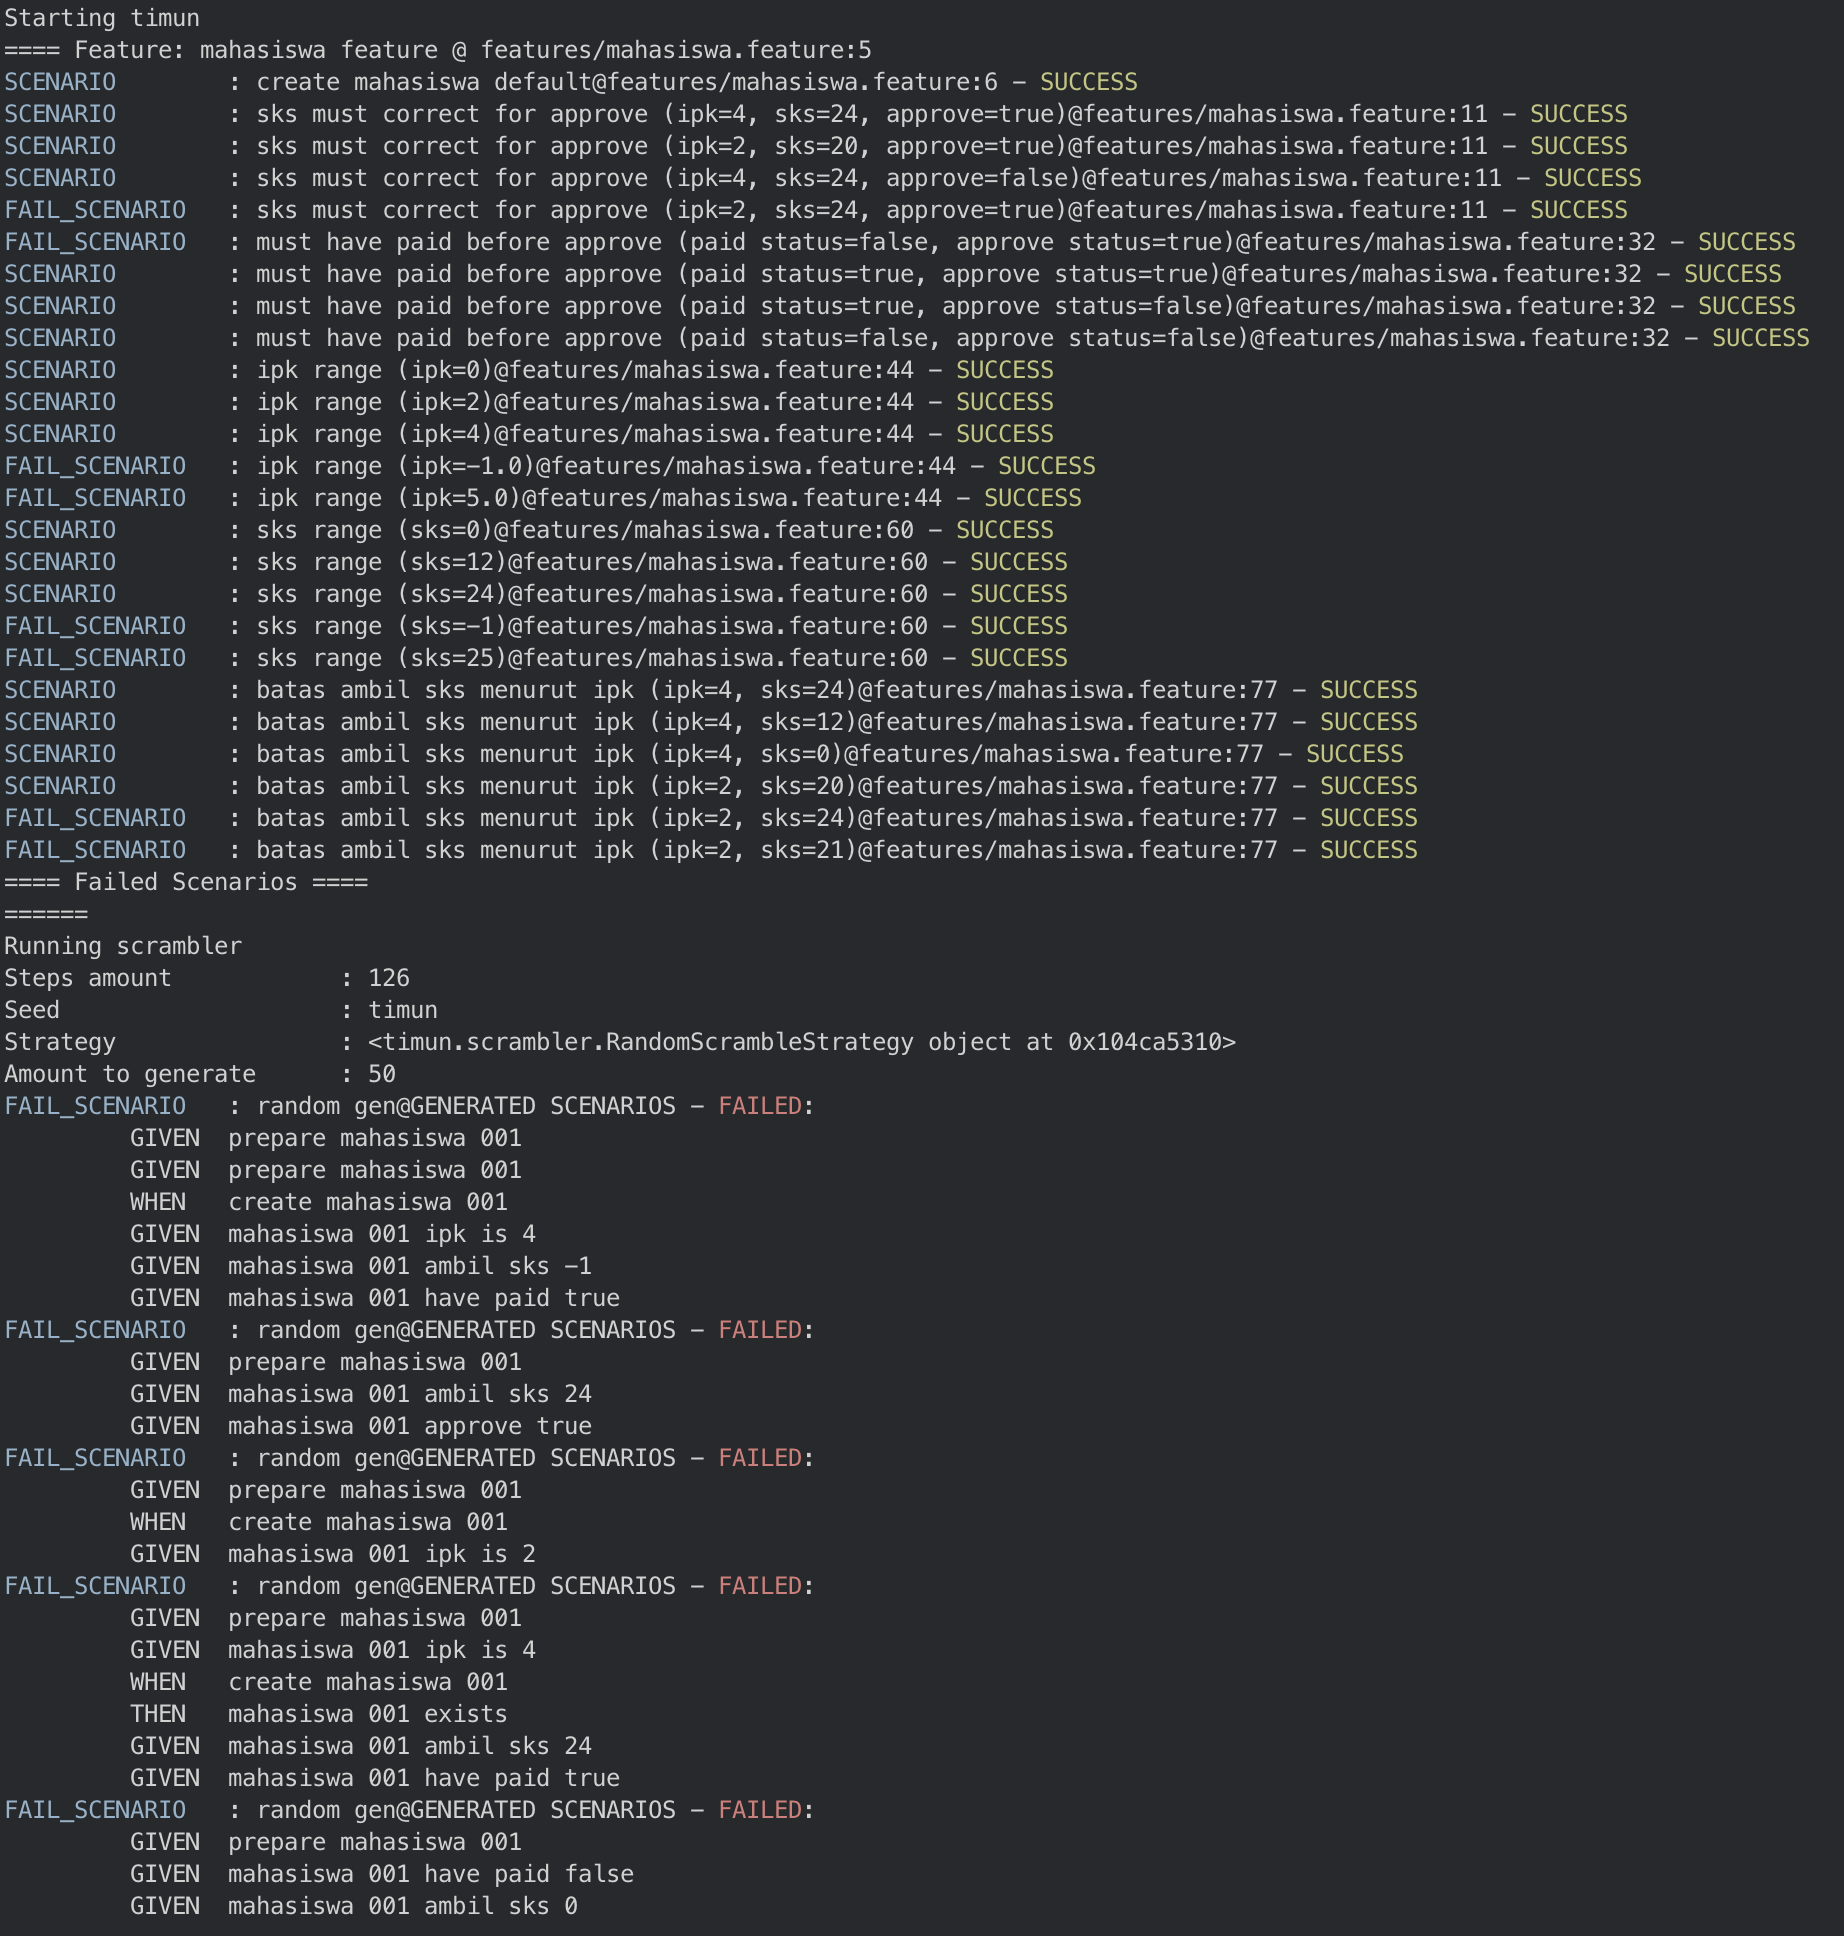
\includegraphics[width=0.8\textwidth]{resources/result.png}
%   \caption{Hasil Pengujian}
%   \label{dia:test-result}
% \end{figure}
\begin{lstlisting}[language=testresult]
Starting timun
==== Feature: mahasiswa feature @ features/mahasiswa.feature:5
SCENARIO	: create mahasiswa default@features/mahasiswa.feature:6 - SUCCESS
FAIL_SCENARIO	: create mahasiswa fail@features/mahasiswa.feature:11 - SUCCESS
SCENARIO	: sks must correct for approve (ipk=4, sks=24, approve=true)@features/mahasiswa.feature:16 - SUCCESS
SCENARIO	: sks must correct for approve (ipk=2, sks=20, approve=true)@features/mahasiswa.feature:16 - SUCCESS
SCENARIO	: sks must correct for approve (ipk=4, sks=24, approve=false)@features/mahasiswa.feature:16 - SUCCESS
FAIL_SCENARIO	: sks must correct for approve (ipk=2, sks=24, approve=true)@features/mahasiswa.feature:16 - SUCCESS
FAIL_SCENARIO	: must have paid before approve (paid status=false, approve status=true)@features/mahasiswa.feature:37 - SUCCESS
SCENARIO	: must have paid before approve (paid status=true, approve status=true)@features/mahasiswa.feature:37 - SUCCESS
SCENARIO	: must have paid before approve (paid status=true, approve status=false)@features/mahasiswa.feature:37 - SUCCESS
SCENARIO	: must have paid before approve (paid status=false, approve status=false)@features/mahasiswa.feature:37 - SUCCESS
SCENARIO	: ipk range (ipk=0)@features/mahasiswa.feature:49 - SUCCESS
SCENARIO	: ipk range (ipk=2)@features/mahasiswa.feature:49 - SUCCESS
SCENARIO	: ipk range (ipk=4)@features/mahasiswa.feature:49 - SUCCESS
FAIL_SCENARIO	: ipk range (ipk=-1.0)@features/mahasiswa.feature:49 - SUCCESS
FAIL_SCENARIO	: ipk range (ipk=5.0)@features/mahasiswa.feature:49 - SUCCESS
SCENARIO	: sks range (sks=0)@features/mahasiswa.feature:65 - SUCCESS
SCENARIO	: sks range (sks=12)@features/mahasiswa.feature:65 - SUCCESS
SCENARIO	: sks range (sks=24)@features/mahasiswa.feature:65 - SUCCESS
FAIL_SCENARIO	: sks range (sks=-1)@features/mahasiswa.feature:65 - SUCCESS
FAIL_SCENARIO	: sks range (sks=25)@features/mahasiswa.feature:65 - SUCCESS
SCENARIO	: batas ambil sks menurut ipk (ipk=4, sks=24)@features/mahasiswa.feature:82 - SUCCESS
SCENARIO	: batas ambil sks menurut ipk (ipk=4, sks=12)@features/mahasiswa.feature:82 - SUCCESS
SCENARIO	: batas ambil sks menurut ipk (ipk=4, sks=0)@features/mahasiswa.feature:82 - SUCCESS
SCENARIO	: batas ambil sks menurut ipk (ipk=2, sks=20)@features/mahasiswa.feature:82 - SUCCESS
FAIL_SCENARIO	: batas ambil sks menurut ipk (ipk=2, sks=24)@features/mahasiswa.feature:82 - SUCCESS
FAIL_SCENARIO	: batas ambil sks menurut ipk (ipk=2, sks=21)@features/mahasiswa.feature:82 - SUCCESS
==== Failed Scenarios ====
======
Running scrambler
Steps amount		: 129
Seed			: .
Strategy		: <timun.scrambler.RandomScrambleStrategy object at 0x10897d2e0>
Amount to generate	: 50
FAIL_SCENARIO	: random gen@GENERATED SCENARIOS - FAILED:
	 GIVEN	prepare mahasiswa 001
	 GIVEN	mahasiswa 001 ambil sks -1
	 GIVEN	mahasiswa 001 ambil sks 20
	 WHEN	create mahasiswa 001
	 THEN	mahasiswa 001 exists
	 GIVEN	prepare mahasiswa 001
FAIL_SCENARIO	: random gen@GENERATED SCENARIOS - FAILED:
	 GIVEN	prepare mahasiswa 001
	 WHEN	create mahasiswa 001
	 THEN	mahasiswa 001 exists
FAIL_SCENARIO	: random gen@GENERATED SCENARIOS - FAILED:
	 GIVEN	prepare mahasiswa 001
	 GIVEN	prepare mahasiswa 001
	 WHEN	create mahasiswa 001
	 GIVEN	mahasiswa 001 approve false
	 THEN	mahasiswa 001 exists
\end{lstlisting}


\subsection{Analisa Hasil Validasi}

Pada paparan hasil validasi diatas, fitur representasi kegagalan ditampilkan pada kode baris 11-14,
32-43, 59-62, 77-80, 94-97 dan hasil eksekusinya terdapat pada hasil baris 4, 16-17, 21-22, 27-28.
Fitur kemampuan menyatakan variansi ditampikan pada kode baris 1-3 dan 37-46, sementara hasil eksekusi
terdapat pada hasil baris 9-12.

Fitur pengacakan skenario ditampilkan pada hasil baris 31-52. Dapat dilihat bahwa dari 50 skenario yang dibangkitkan,
terdapat 3 skenario yang tidak lulus (skenario yang dibangkitkan seharusnya gagal saat dijalankan namun skenario ini tidak gagal).
Ada beberapa penyebab skenario ini tidak lulus.
Pertama kakas pembangkitan menghasilkan skenario yang telah dinyatakan benar pada kode gherkin sehingga menghasilkan \textit{false negative}.
Kedua kakas pembangkitan menghasilkan skenario dengan alur logika yang tidak berurut (given-when-then), pada beberapa \textit{seed}
lain kakas juga tidak menghasilkan skenario yang memiliki step \texttt{then} sehingga tidak ada pengecekan yang dilakukan.
Dari beberapa seed yang digunakan, kakas masih belum menghasilkan skenario acak yang menemukan kesalahan logika pada program,
hal ini dapat terjadi karena ukuran program pengujian yang tidak terlalu besar menyebabkan implementasi yang tidak memiliki kelemahan,
kurang banyaknya skenario yang dibangkitkan, atau karena pembangkitan skenario yang belum terlalu efektif.

Pada proses pembuatan kode gherkin, ditemukan kekurangan terhadap rancangan dimana fitur-fitur yang dirancang
tidak dapat berkerjasama dengan baik dalam keadaan tertentu. Fitur ini adalah \emph{fail example} dengan \emph{variable rejecte}
dimana jika digunakan bersamaan akan menghasilkan \emph{double negative} yang menyebabkan skenario pengujian lebih
sulit untuk dipahami dan tidak berjalan sesuai ekspektasi.

Untuk kemudahan, melalui studi lain \cite{dsl_lesson} ditemukan bahwa penggunaan DLS BDD seperti Gherkin walaupun
pada awalnya terlihat menjanjikan namun dalam waktu lama dibutuhkan standarisasi bahasa yang digunakan, karena tiap
orang yang menulis kasus pengujian dapat mendeskripsikan kasus dengan cara yang berbeda-beda. \emph{User} yang
akan menggunakan kakas pengujian juga memerlukan pelatihan dalam penggunaan kerangka pikir dan kakas untuk menghasilkan
kasus pengujian yang baik.

% Dari hasil diatas dapat dilihat bahwa fitur pengujian biasa seperti fitur dari gherkin,
% representasi kegagalan, dan deklarasi variabel telah bejalan dengan baik.
% Fitur-fitur ini membantu penulis untuk menemukan kekurangan dalam pengujian ataupun implementasi selama
% penulisan.
% Namun selama
% pengembangan kakas ditemukan bahwa fitur deklarasi variabel tidak dapat berkerja sama dengan
% fitur representasi kegagalan menggunakan \texttt{Fail Example Scenario Outline}, dimana
% saat menggunakan deklarasi variabel dengan tabel \texttt{Variable Rejected} dan tabel \texttt{Fail Example}
% terjadi negatif ganda dan sulit untuk dimengerti. Hal ini menyebabkan fitur tabel \texttt{Variable} tidak dapat
% digunakan besamaan dengan fitur \texttt{Scenario Outline}.

% Untuk fitur pengacakan skenario masih banyak menghasilkan false positive dan false negative karena
% pembangkitan skenario acak yang masih sangat simpel dan belum mengikuti urutan yang seharusnya.
    % \chapter{Penutup}

\section{Kesimpulan}

% Dalam pengembangan perangkat lunak, masih sulit dilakukan pengujian terhadap kelemahan keamanan berjenis \emph{Business Logic Error}.
% Hal ini terjadi karena kelemahan jenis ini membutuhkan pengoperasian perangkat lunak secara valid dengan langkah-langkah tertentu, dimana
% tiap langkah tersebut adalah langkah yang valid yang menyebabkan pengujian secara otomatis menjadi mustahil.

% BDD memberikan kumpulan pengetahuan langkah-langah \emph{business rule} yang mungkin terjadi terhadap perangkat lunak. Pengetahuan ini
% dapat dimanfaatkan untuk melakukan pengujian secara otomatis dengan membangkitkan skenario-skenario acak.
% BDD juga dapat ditambahkan fitur-fitur baru secara bahasa yang dapat mempermudah penguji untuk melakukan \emph{refactor} terhadap
% skenario pengujian, dan menambahkan skenario baru.

Dari pengerjaan tugas akhir ini dapat ditarik beberapa kesimpulan.

\begin{enumerate}
      \item Pengujian keamanan berbeda dengan pengujian fungsionalitas dimana pengujian fungsionalitas hanya menguji apakah fungsionalitas
            telah diimplementasikan dan berjalan dengan baik. Sementara pengujian keamanan menguji bahwa tidak ada celah-celah keamanan
            yang terbentuk. Pengujian keamanan sering tidak optimal karena \textit{programmer} biasanya hanya melakukan pengujian
            fungsionalitas saja.

      \item Pengujian sulit dilakukan walaupun telah menggunakan kakas sekalipun karena kakas pengujian masih memiliki banyak kekurangan
            yang menyebabkan programmer menjadi terdorong untuk tidak melakukan pengujian dengan baik. Untuk pengujian
            keamanan khususnya, kakas yang ada pada saat ini jauh berbeda dan tidak dapat bekerjasama dengan kakas
            yang digunakan pada pengujian fungsionalitas. Perbedaan ini menyebabkan adanya pengetahuan domain program
            yang dapat tidak tersampaikan saat dilakukan pengujian dari dua sisi.

      \item Hal-hal yang dibutuhkan pada kerangka pengujian keamanan, khususnya \textit{Business Logic Error}, adalah fitur
            yang dapat mempermudah pengujian keamanan. Fitur-fitur ini adalah representasi kegagalan, kemampuan menyatakan variansi,
            dan pengacakan skenario. Dua fitur pertama membantu dalam melakukan \textit{refactor} terhadap kode pengujian sehingga
            tidak terjadi duplikasi, dan fitur terakhir membantu penguji dalam menemukan kelemahan keamanan baru.
\end{enumerate}

\section{Saran}

Dari dua poin fitur pertama, pada pengujian ditemukan bahwa fitur \texttt{Fail Scenario} tidak dapat bekerjasama dengan fitur
\textit{Variabel Rejected}. Pada intinya saat kedua fitur ini digunakan akan menyebabkan negasi ganda terhadap skenario
dasar yang dihasilkan. Negasi ganda ini menyebabkan skenario yang dihasilkan tidak intuitif dan sulit untuk dilogikakan
oleh programmer. Solusi yang dapat dilakukan adalah dengan membatasi fitur variabel hanya dapat digunakan pada skenario
biasa, atau dengan melakukan rancangan kembali agar dapat menghasilkan desain yang lebih baik.

Pada implementasi, fitur pengacakan skenario menghasilkan skenario yang benar-benar acak tanpa ada aturan tertentu.
Hal ini menyebabkan skenario yang dihasilkan bernilai \textit{false negative}. Jumlah step pada program pengujian
yang sedikit menyebabkan tidak ditemukannya kelemahan terhadap program pengujian. Solusi yang dapat dilakukan
adalah dengan menggunakan algoritma pembangkitan skenario yang lebih kompleks sehingga dihasilkan skenario yang lebih efektif,
dan pengujian kakas juga dilakukan dengan program yang lebih besar dan komplek.

Untuk validasi kedepannya program yang akan diuji dapat dibuat lebih besar dan lebih kompleks sehingga dapat dilihat apakah
solusi yang didesain dapat bekerja dengan efektif untuk program yang besar.
    %----------------------------------------------------------------%

    % Daftar pustaka
    \printbibliography

    % Index
    \appendix

    % \addcontentsline{toc}{part}{Lampiran}
    % \part*{Lampiran}

    % \chapter{Instrumen Pengujian}
    % \chapter{Rincian Kasus Uji}

\end{document}
